
\section{Organizacja pracy grupy}
Członkowie grupy są ludźmi. Jako ludzie, szukamy na około, tracimy główny wątek 
dyskusji, przywiązujemy się do naszych pomysłów. Nawet jeśli bardzo się staramy,
żeby utrzymać koncentrację i „pozostać na torze”, nie możemy zmienić faktu, że 
jesteśmy indywidualnościami o różnych punktach widzenia. Podczas dyskusji, 
każdy z członków grupy powinien mieć okazję do przedstawienia swoich propozycji 
rozwiązań oraz oceny innych alternatyw. W większości przypadków dochodzi do tak 
zwanej ,,burzy mózgów''. Bardzo dużo osób obawia się, że proces wymknie się spod
kontroli i zostanie zatracony sens dyskusji. Niemniej jednak, coś co wydaje się 
być chaosem, może okazać się wstępem do kreatywności. Dlatego w modelu 
podejmowania decyzji grupowej powinien być czas na tak zwaną ,,strefę
rozbieżną'' oraz ,,strefę zbieżną'', a pomiędzy nimi ,,strefę jęku''
\cite{Kaner1996}. Są to elementy, które większość isniejących modeli pomija, a
tak naprawdę to właśnie dyskusja jest kluczem prowadzącym do osiągnięcia
konsensus.

Strefa rozbieżna to miejsce na myślenie w coraz to szerszym zakresie. Na samym 
początku grupa przedstawia oczywiste lub dobrze znane (na przykład z 
poprzednich problemów) rozwiązania. Jeśli okaże się to wystarczające to 
wyszukiwanie alternatyw może się zakończyć w tym miejscu. Jednakże istnieją 
problemy, na które nie ma prostej odpowiedzi i grupa musi wyjść poza pewne ramy 
w poszukiwaniu szerszego spektrum możliwości. To jest miejsce, do którego wiele 
grup nie dociera. Boimy się wychodzić poza utarte schematy, bo możemy zostać 
skrytykowani lub, w najlepszym wypadku, zignorowaniu. To jest również jedno z 
tych miejsc, w których idealnie sprawdza się system informatyczny, w którym 
zapewniona jest anonimowość przedstawianych rozwiązań.

Teoretycznie, w pewnym momencie czasu, grupa sama powinna zacząć myśleć w 
kierunku uporządkowania dyskusji i wyboru ostatecznych rozwiązań, czyli  przejść
do ,,strefy zbieżnej''. Niestety, w prawdziwym życiu jest inaczej. W praktyce,
przejście ze strefy wyrażania swoich propozycji do strefy rozumienia perspektyw 
pozostałych członków grupy jest bardzo trudne. Ludzie mogą czuć się przeciążeni,
zdezorientowani, zniechęceni. Mogą pojawić się stwierdzenia o utknięciu w 
miejscu, o traceniu czasu, osoby  z silniejszą pozycją mogą nakłaniać do 
zakończenia procesu i wybraniu ich opcji.

Członkowie grupy, zanim zaczną rozumieć punkt widzenia innych członków, muszą 
przejść przez fazę walki o integrację nowych, innych podejść do problemu ze 
swoim samym. Jest to tak zwana „strefa jęku”. Jest to miejsce na dyskusje, a 
nawet kłótnie. Sam fakt świadomości, że w procesie jest miejsce na wymianę zdań, 
może znacząco przyczynić się do osiągnięcia konsensusu przez grupę.

\section{Zasada działania}
Zaproponowany w tej pracy system wspomagania decyzji grupowej ma za zadanie
poprowadzić grupę przez cały proces oraz ułatwić osiągnięcie konsensusu i
wybranie optymalnego rozwiązania. W związku z opisaną powyżej organizacją pracy
grupy, ważnym elementem systemu jest moduł dyskusji. Eksperci mają możliwość
przedstawiać swoje alternatywy oraz, oprócz zwykłego głosowania, wyrażać opinię
i rozmawiać na temat problemu i rozwiązań. Dzięki temu, grupa może poczuć się
jak na rzeczywistym spotkaniu. Prowadzi to do kolejnego założenia.

System umożliwia dynamiczną dyskusję nad problemem bez konieczności gromadzenia 
ekspertów w jednym miejscu i czasie. Aby uczestniczyć w podjęciu decyzji 
wymagane jest tylko urządzenie z dostępem do internetu oraz przeglądarką 
internetową. Zastosowanie najnowszych technologii mobilnych rozszerza możliwości
podejmowania decyzji, na przykład możliwe jest osiągnięcie konsensusu wśród 
ekspertów rozlokowanych w różnych krajach i strefach czasowych.

Szczegółowy opis działania systemu na przykładach opisany jest w kolejnym 
rozdziale, natomiast poniżej przedstawiony został model teoretyczny 
wykorzystujący techniki przedstawione wcześniej.

\section{Model teoretyczny}
Opisywany model teoretyczny bazuje na modelu przedstawionym w pracy Alonso et
al. \cite{Alonso2010} oraz wprowadza kilka udoskonaleń.

Jednym z nich jest zrezygnowanie z podejścia iteracyjnego. Oznacza to dużo
większą dynamikę oraz naturalność procesu. W klasycznym podejściu, system czeka
aż wszyscy eksperci biorący udział w procesie wprowadzą swoje preferencje
względem alternatyw, a sam zbiór ekspertów jest stały. W przypadku braku
informacji od któregoś z członków zespołu cały proces wspomagania decyzji
zostaje wstrzymany. 
Lepszym rozwiązaniem jest uruchomienie etapów schematu modelu w momencie
otrzymania pierwszego, nawet niepełnego, zbioru preferencji od jednego z
ekspertów. System obliczając poziom konsensusu bierze pod uwagę ilość
głosujących ekspertów do ilości wszystkich ekspertów biorących udział w
procesie. Pozwala to zapewnić płynność procesu oraz ułatwia dynamiczne
zarządzanie zbiorem ekspertów.

Zrezygnowanie z podejścia iteracyjnego w naturalny sposób pociąga kolejną
modyfikację. W klasycznych modelach na początku ustalana jest maksymalna liczba
iteracji, po której system powinien zakończyć działanie bezwzględu na wynik.
Ze względu na specyfikę zagadnienia, system powinien jedynie wspomagać grupę i
sugerować działania, ale nie podejmować decyzji samodzielnie. To zespół powinien
decydować, czy osiągnięty konsensus jest satysfakcjonujący czy nie, dlatego
proces wspierania decyzji domyślnie jest nieskończony w czasie.

Struktura proponowanego modelu grupowego podejmowania decyzji składa się z
sześciu etapów opisanych w kolejnych punktach:
\begin{itemize}
  \item etap unifikowania,
  \item etap selekcji,
  \item etap konsensusu,
  \item etap dynamicznego wyboru alternatyw,
  \item etap informacji zwrotnej,
  \item etap dynamicznej selekcji ekspertów.
\end{itemize}

\begin{figure}[!htbp]
  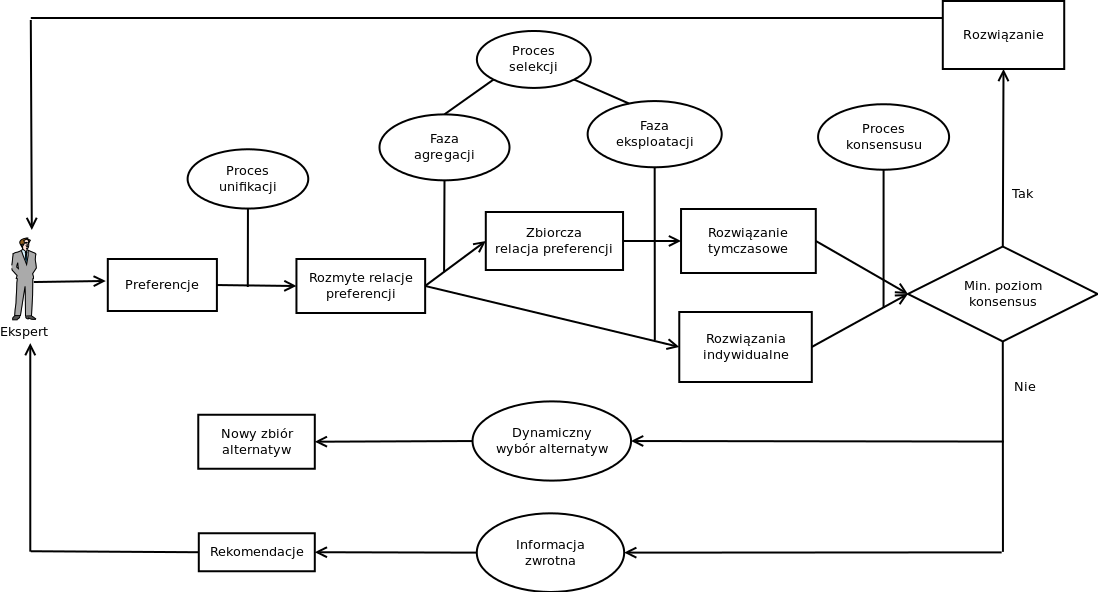
\includegraphics[width=\linewidth]
    {chapters/tdmmodel/model_schema}
  \caption{Schemat modelu}
  \label{fig:model_schema}
\end{figure}

\subsection{Etap unifikowania}
Aby sprostać wymaganiom użytkowników oraz zapewnić duży stopień swobody w
wyrażaniu swoich preferencji, eksperci mogą wprowadzać swoje oceny na temat
alternatyw przy pomocy dowolnie przez siebie wybranej metody wprowadzania
preferencji opisanej w rozdziale na temat sposobów prezentacji preferencji. W
związku z tym, konieczne jest zunifikowanie uzyskanych informacji przed
przejściem do dalszych etapów. Ze względu na użyteczność i wygodę w dalszym
przetwarzaniu informacji, szczególnie przy agregacji ocen ekspertów w ocenę
zbiorczą, do reprezentacji preferencji w dalszych etapach wybrano rozmytą
relację preferencji \cite{Ma2006}. Aby jednak było możliwe zamienianie
poszczególnych metod na relację rozmytą, potrzebne są funkcje transformacji.

\subsubsection{Funkcja użyteczności a relacja rozmyta}
W przypadku funkcji użyteczności zakłada się, że każdy ekspert $e_k$ podaje
swoje preferencje dla zbioru alternatyw $\mathcal{X}$ jako zbiór wartości
użyteczności $U^k = \{ u^k_i; i=1,\dotsc,n\}, u^k_i \in [0,1]$, gdzie
$u^k_i$ reprezentuje wartość użyteczności alternatywy $x_i$ daną przez eksperta
$e_k$. Dla każdego zbioru $U^k$ bez straty ogólności, można założyć, że im
wyższa wartość tym bardziej dana alternatywa odpowiada ekspertowi.

Dowolna możliwa funkcja transformacji $f$ musi ustalić dla eksperta $e_k$ jego
stopień preferencji alternatywy $x_i$ nad $x_j$ ($p^k_{ij}$) tylko w zależności
od wartości $u^k_i$ oraz $u^k_j$, to znaczy 
\begin{equation}
p^k_{ij} = h(u^k_i, u^k_j).
\end{equation}
Funkcja transformacji $f$ musi zakładać również, że większa wartość $u^k_i$
pociąga większą wartość $p^k_{ij}$, a większa $u^k_j$ to mniejsza $p^k_{ij}.$

\begin{theorem}
Dla każdego zbioru wartości użyteczności $U^k = \{ u^k_1, \dotsc, u^k_n \}$ nad
zbiorem alternatyw $\mathcal{X} = x_1, \dotsc, x_n\}$, stopień preferencji
alternatywy $x_i$ nad $x_j$ ($p^k_{ij}$) otrzymywany jest ze współczynnika
$^{u^k_i}/_{u^k_j}$ przy użyciu następującej funkcji transformacji:
\begin{equation}
p^k_{ij} = f(u^k_i, u^k_j) =
  \left\{ 
	\begin{array}{ll}
	  \frac{s(u^k_i)}{s(u^k_i) + s(u^k_j)} , & \quad \textrm{jeżeli } (u^k_i,u^k_j)
	  \neq (0,0) ,
	  \\
      \frac{1}{2} , & \quad \textrm{jeżeli } (u^k_i,u^k_j) = (0,0),
  	\end{array} 
  \right. (i \neq j) .
\end{equation}
gdzie $s : [0,1] \rightarrow \mathbb{R}^+$ jest dowolną niemalejącą i ciągłą
funkcją spełniającą $s(0) = 0.$
\end{theorem}

Przykładowa funkcja spełniająca powyższe twierdzenie zaproponowana w
\cite{Chiclana1996} oraz wykorzystywana w przedstawianym systemie wygląda
następująco:
\begin{equation}
f^1(u^k_i,u^k_j) = \frac{(u^k_i)^2}{(u^k_i)^2 + (u^k_j)^2}
\end{equation}

\subsubsection{Uporządkowanie alternatyw a relacja rozmyta}
W tym przypadku, ekspert $e_k$ podaje swoje preferencje jako uporządkowanie
alternatyw $O^k = \{o^k(1), \dotsc, o^k(n)\}$. Dla każdego zbioru $O^k$ bez
straty ogólności, można założyć, że im mniejsza pozycja alternatywy w
uporządkowaniu tym większa satysfakcja eksperta. Dla przykładu, uporządkowanie
zbioru alternatyw $\mathcal{X} = \{x_1,x_2,x_3,x_4\}$ przez eksperta $e_k$ to
$O^k = \{3,1,4,2\}.$ Oznacza to, że alternatywa $x_2$ jest najlepsza dla
eksperta, a $x_3$ najgorsza.

Dowolna możliwa funkcja transformacji $f$ musi ustalić dla eksperta $e_k$ jego
stopień preferencji alternatywy $x_i$ nad $x_j$ ($p^k_{ij}$) tylko w zależności
od wartości $o^k(i)$ oraz $o^k(j)$, to znaczy
\begin{equation}
p^k_{ij} = f(o^k(i), o^k(j)).
\end{equation}
Funkcja transformacji $f$ musi zakładać również, że większa wartość $o^k(i)$
pociąga mniejszą wartość $p^k_{ij}$, a większa $o^k(j)$ to większa $p^k_{ij}$.

\begin{theorem}
Dla każdego uporządkowania alternatyw $O^k = \{o^k(1), \dotsc, o^k(n)\}$ nad
zbiorem alternatyw $\mathcal{X} = \{x_1,\dotsc,x_n\}$, stopień preferencji
alternatywy $x_i$ nad $x_j$ ($p^k_{ij}$) otrzymywany jest przy użyciu
następującej funkcji transformacji:
\begin{equation}
p^k_{ij} = f(o^k(i),o^k(j)) = \frac{1}{2} [1 + F(o^k(j) - o^k(i)) - F(o^k(i) -
o^k(j))].
\end{equation}
gdzie $F$ jest dowolną funkcją niemalejącą.
\end{theorem}

Przykładowa funkcja spełniająca powyższe twierdzenie zaproponowana w
\cite{Chiclana1996} oraz wykorzystywana w przedstawianym systemie wygląda
następująco:
\begin{equation}
f^2(o^k(i),o^k(j)) = \frac{1}{2}(1 + \frac{o^k(j) - o^k(i) }{n-1}).
\end{equation}

\subsubsection{Multiplikatywna relacja preferencji a relacja rozmyta}
Ekspert $e_k$ podaje swoje preferencje poprzez multiplikatywną relację
preferencji $A^k = [a^k_{ij}]$. W ogólności, zgodnie z propozycją Saaty'ego
\cite{Saaty2000}, jeżeli
$$A' = \{ A^k = [a^k_{ij}] : a^k_{ij} \cdot a^k_{ji} = 1,\;\; a^k_{ij} \in
[^1/_9,9],\;\; k= 1, \dotsc, m \}$$ 
jest multiplikatywną relacją preferencji oraz
$$P' = \{ P^k = [p^k_{ij}] : p^k_{ij} + p^k_{ji} = 1,\;\; p^k_{ij} \in
[0,1],\;\; k= 1, \dotsc, m \}$$
jest rozmytą relacją preferencji, to szukana funkcja transformacji ma postać:
$$F : A' \rightarrow P',\; F(A^k) = P^k \;\; \forall k.$$ 
Ta klasa funkcji jest równoważna klasie funkcji spełniających
$$f : [1/9, 9] \rightarrow [0,1],$$
$$ f(x)+f(1/x)=1 \text{ oraz } f(9)=1.$$
Funkcja $f$ może być zapisana w postaci $f(x) = \frac{1}{2} + h(x)$, co
implikuje $h(x) + h(\frac{1}{x}) = 0 $ oraz $h(9) = \frac{1}{2}.$

Z drugiej strony, ogólne rozwiązanie równania funkcjonalnego $l(x \cdot y) =
l(x) + l(y)$ na przedziale $[1, \infty]$ to $l(z) = C \cdot \ln z, C \in
\mathbb{R}.$
W tej sytuacji, zachodzi $y = \frac{1}{x}$ i podstawiając $x = 1$ dostajemy $0
= h(1) + h(1) = 2 \cdot h(1) = 2 \cdot h(x \cdot y).$ Funkcja $h$ spełnia
$h(x \cdot y) = h(x) + h(y)$, czyli $l(z) = C \cdot \ln z, C \in \mathbb{R}.$
Skoro $h(9) = \frac{1}{2}$, to $C = \frac{1}{2 \cdot \ln 9}$ oraz $h(z) =
\frac{1}{2} \frac{\ln z}{\ln 9} = \frac{1}{2} \log_9 z.$

Podsumowując, w \cite{Chiclana1996} otrzymano następujące twierdzenie:
\begin{theorem}
Dla każdej relacji preferencji $A^k = [a^k_{ij}]$ nad zbiorem alternatyw
$\mathcal{X} = \{x_1,\dotsc,x_n\}$, stopień preferencji alternatywy $x_i$ nad
$x_j$ ($p^k_{ij}$) otrzymywany jest przy użyciu następującej funkcji
transformacji:
\begin{equation}
f^3(a^k_{ij}) = \frac{1}{2}(1 + \log_9 a^k_{ij}).
\end{equation}
\end{theorem}

\subsubsection{Niepełna ocena}
Zazwyczaj modele grupowego podejmowania decyzji zakładają, że ekspert jest
zawsze w stanie podać swoje preferencje względem wszystkich alternatyw. Jest to
bardzo optymistyczne założenie, ponieważ w trakcie trwania dyskusji oraz ze
względu na dynamikę zbioru alternatyw nie zawsze istnieje taka możliwość. Z
braku czasu, niewystarczającej wiedzy lub danych, albo z innych indywidulanych
przyczyn eksperci mogą wyrazić swoje preferencje względem tylko części
alternatyw. W takich sytuacjach mówi się o \emph{niepełnej rozmytej relacji
preferencji}.

W pracy Alonso, Cabrerizo et al. \cite{Alonso2009} została przedstawiona metoda
estymacji brakujących wartości. Zapewnia ona addytywną konsystencję z
preferencjami podanymi przez eksperta. Jest to iteracyjna procerdura, która w
całości została zaadoptowana w tej pracy.

\subsection{Proces selekcji: agregacja}
Jest to faza, w której definiowana jest zbiorcza rozmyta relacja preferencji
$P^c = [p^c_{ij}]$, otrzymana poprzez agregację wszystkich indywidualnych
rozmytych relacji preferencji otrzymanych w procesie unifikacji $\{ P^1, P^2,
\dotsc, P^m \}$. Każda wartość $p^c_{ij} \in [0,1]$ reprezentuje stopień
preferencji alternatywy $x_i$ nad $x_j$ według opinii większości ekspertów.
Tradycyjnie, większość oznacza pewną liczbę progową. W tym przypadku, stosowana
jest rozmyta większość wyrażona przez rozmyty kwantyfikator lingwistyczny.

Każda wartość $p^c_{ij}$ jest obliczana przy pomocy operatora agregacji OWA.
Operator OWA odzwierciedla rozmytą większość obliczając wektor wag przy pomocy
kwantyfikatora rozmytego \cite{Peneva2007}. Zatem zbiorcza rozmyta relacja
preferencji otrzymywana jest w następujący sposób:
\begin{equation}
p^c_{ij} = \Phi_Q(p^1_{ij}, \dotsc, p^m_{ij}).
\end{equation}
gdzie $Q$ jest rozmytym kwantyfikatorem użytym do obliczenia wektora wag dla
operatora OWA $\Phi_Q$.

\subsection{Proces selekcji: eksploatacja}
W tej fazie przekształcana jest globalna informacja o alternatywach w globalny
ranking, z której można uzyskać zbiór rozwiązań. Globalny ranking uzyskuje się
poprzez użycie dwóch stopni wyboru alternatyw
\cite{Herrera1996a,Campanella2011}:
\begin{itemize}
  \item kwantyfikowany stopień dominacji QGDD (ang. \textit{quantifier guided
  dominance degree}) oraz
  \item kwantyfikowany stopień nie-dominacji QGNDD (ang. \textit{quantifier
  guided non dominance degree}).
\end{itemize}

Kwantyfikowany stopień dominacji $QGDD_i$ to wielkość dominacji jaką posiada
alternatywa $x_i$ nad pozostałymi w sensie rozmytej większości:
\begin{equation}
QGDD_i = \Phi_Q(p^c_{i1}, p^c_{i2}, \dotsc, p^c_{i(i-1)},p^c_{i(i+1)}, \dotsc,
p^c_{i \cdot n}).
\end{equation}
Ta miara pozwala na zdefiniowanie zbioru dominujących alternatyw z maksymalnym
stopniem dominacji:
\begin{equation}
X^{QGDD} = \{ x_i \in \mathcal{X} : QGDD_i = \sup_{x_j \in \mathcal{X}} QGDD_j
\}.
\end{equation}

Kwantyfikowany stopień nie-dominacji $QGNDD_i$ podaje stopień w jakim każda
alternatywa nie jest zdominowana przez pozostałe alternatywy w sensie rozmytej
większości:
\begin{equation}
QDNDD_i = \Phi_Q(\neg(p^s_{1i}), \neg(p^s_{2i}), \dotsc,
\neg(p^s_{(i-1)i}), \neg(p^s_{(i+1)i}), \dotsc, \neg(p^s_{n \cdot i})).
\end{equation}
gdzie
$p^s_{ji} = 
  \left\{ 
	\begin{array}{ll}
	  0 				  & \quad \textrm{jeżeli } p^c_{ji} < p^c_{ij} \\
      p^c_{ji} - p^c_{ij} & \quad \textrm{jeżeli } p^c_{ji} \geq p^c_{ij}
  	\end{array} 
  \right.
$
reprezentuje stopień, w jakim alternatywa $x_i$ jest bezwzględnie zdominowana
przez $x_j$.

Ta miara pozwala na zdefiniowanie zbioru niezdominowanych alternatyw:
\begin{equation}
X^{QGNDD} = \{ x_i \in \mathcal{X} : QGNDD_i = \sup_{x_j \in \mathcal{X}}
QGNDD_j
\}.
\end{equation}

Po zastosowaniu tych dwóch stopni można wyznaczyć rozwiązanie w postaci
\begin{equation}
X_{sol} = X^{QGDD} \cap X^{QGNDD}.
\end{equation}

\subsection{Proces konsensusu}
Jest to proces w trakcie którego znalezione rozwiązanie $X_{sol}$ jest
porównywane z indywidualnymi rozwiązaniami ekspertów. Dzięki temu możliwe jest
zmierzenie konsensusu, czyli w jakim stopniu eksperci zgadzają się z
zaproponowanym rozwiązaniem. W prezentowanym modelu grupowego podejmowania
decyzji, wykorzystywany jest proces konsensusu zaprezentowany w
\cite{Herrera1995}. Model ten zawiera następujące główne cechy:
\begin{itemize}
  \item Jest oparty na dwóch kryteriach konsensusu: globalna miara konsensusu
  nad zbiorem alternatyw $\mathcal{X}$ oznaczana jako $C_{\mathcal{X}}$ oraz
  miara bliskości każdego eksperta nad $\mathcal{X}$ oznaczanych jako
  $P^k_{\mathcal{X}}$.
  \item Oba kryteria konsensusu są definiowane przez porównanie indywidualnych
  rozwiązań z globalnym rozwiązaniem, używając jako kryterium porównawczego
  pozycji alternatyw w każdym z rozwiązań.
\end{itemize}

Początkowo zakłada się, że w każdym nietrywialnym problemie grupowego
podejmowania decyzji, eksperci nie są zgodni w swoich opiniach i osiągnięcie
konsensusu musi być traktowane jako proces iteracyjny. Oznacza to, że
porozumienie można uzyskać dopiero po kilku rundach konsultacji. W każdej
rundzie system oblicza obie miary, konsensusu oraz bliskości. Miara konsensusu
ocenia istniejące porozumienie wśród ekspertów, natomiast miary bliskości są
wykorzystywane w procesie informacji zwrotnej wspierając w ten sposób fazę
dyskusji procesu konsensusu.

Głównym problemem jest znalezienie sposobu, aby indywidualne rankingi
poszczególnych ekspertów były zbieżne, a zatem, jak wspierać ekspertów w
uzyskaniu porozumienia. W tym celu, ustalany jest z góry poziom konsensusu (CL)
jaki muszą uzyskać eksperci w danym przypadku. Kiedy miara konsensusu osiągnie
ustalony poziom, wtedy proces podejmowania decyzji jest zakończony i jest
prezentowane wybrane rozwiązanie. Jeżeli nie osiągnięto odpowiedniego poziomu
konsensusu, preferencje ekspertów muszą ulec modyfikacji.

\subsection{Proces konsensusu: wskaźniki konsensusu}
Każdy z parametrów konsensusu wymaga wykorzystania funkcji odległości
$d(V^k,$ $V^c)$, aby uzyskać poziom porozumienia pomiędzy indywidualnym
rozwiązaniem eksperta $e_k$, $V^k = (V^k_1, \dotsc, V^k_n)$, gdzie $V^k_i$ to
pozycja alternatywy $x_i$ w rozwiązaniu $k-tego$ eksperta oraz globalnym
rozwiązaniem $V^c = (V^c_1, \dotsc, V^c_n)$, gdzie $V^c_i$ to pozycja
alternatywy $x_i$ w globalnym rozwiązaniu. W tym celu można korzystać z wielu
różnych metod, takich jak na przykład odległość euklidesowa albo kosinus i sinus
kąta między wektorami. Zazwyczaj proponowane metody bazują nie tylko na pozycji,
ale również na wartości stopnia wyboru, W tym modelu wykorzystywana jest
tylko rzeczywista pozycja w wektorze preferencji, ponieważ identyczne rankingi
alternatyw mogą mieć przypisane różne wektory stopni wyboru. Jako przykład
rozpatrzone zostaną dwa wektor uporządkowania alternatyw: $[(3;0.8), (1;1),
(2;0.9), (4;0.4)]$ oraz $[(3;0.4), (1;0.8), (2;0.5), (4;0.1)]$, gdzie $(3; 0.4)$
w drugim wektorze oznacza, że pierwsza alternatywa jest na trzeciej pozycji ze
stopniem wyboru $0.4$. Zatem, w obu wektorach pierwsza alternatywa jest na
trzeciej pozycji, ale w każdym z innym stopniem wyboru. Gdyby używać stopni
wyboru przy porównywaniu konsensusu to można by mówić o pełnym konsensusie, co
jest w rzeczywistości bardzo trudne do osiągnięcia. Tym bardziej, że w systemie
wykorzystywane są różne metody wprowadzania preferencji.

Zatem, określanie wskaźników konsensusu odbywa się w następujący sposób
\cite{Herrera-Viedma2002}:
\begin{enumerate}
  \item Obliczana jest bliskość każdego eksperta dla każdej alternatywy
  porównując pozycję danej alternatywy w rozwiązaniu eksperta oraz zbiorczym.
  Porównanie to jest wykonywane przy pomocy funkcji $p_k(x_i) = p(V^k,V^c)(x_i)
  = f(|V^c_i - V^k_i|)$ odzwierciedlającej bliskość obu pozycji. Oznacza to, że
  taka funkcja musi być funkcją rosnącą. Jako funkcję ogólną przyjmuje się
  $f(x) = (a \cdot x)^b, 1 \geq b \geq 0$, a w tym szczególnym przypadku
  rozważana będzie funkcja z $a = \frac{1}{n-1}$:
  \begin{equation}
  p_k(x_i) = p(V^k,V^c)(x_i) = f(|V^c_i - V^k_i|) = (\frac{|V^c_i -
  V^k_i|}{n-1})^b \in [0,1].
  \end{equation}
  Parametr $b$ kontroluje rygorystyczność procesu, to znaczy, jeżeli wartość $b$
  jest bliska $1$, to zmniejsza się rygorystyczność i tym samym, liczba rund.
  Najczęściej przyjmowane wartości to: $0.5, 0.7, 0.9, 1$.
  
  \item Obliczany jest stopień konsensusu wszystkich ekspertów dla każdej
  alternatywy:
  \begin{equation}
  C(x_i) = 1 - \sum_{k=1}^{m} \frac{p_k(x_i)}{m}.
  \end{equation}
  
  \item Miara konsensusu nad zbiorem alternatyw $C_{\mathcal{X}}$ obliczana jest
  przez agregację stopni konsensusu z poprzedniego kroku. Agregacja
  robiona jest w taki sposób, aby stopnie konsensusu dla wstępnego zbioru
  rozwiązań $\mathcal{X}_{sol}$ miały większą wagę. Operator agregacji, który
  pozwala na tego typu operację to S-OWA OR-LIKE zdefiniowany przez Yagera i
  Fileva.
  \begin{equation}
  \begin{split}
  C_{\mathcal{X}} &= S_{OWA \; OR\_LIKE}(\{ C(x_s); x_s \in
  \mathcal{X}_{sol}\}, \{ C(x_t); x_t \in \mathcal{X} - \mathcal{X}_{sol} \}) =
  \\ 
  &= (1 - \beta)\cdot \sum_{t=1}^{v} \frac{C(x_t)}{v} + \beta \cdot
  \sum_{s=1}^{\gamma} \frac{C(x_s)}{\gamma},
  \end{split}
  \end{equation}
  gdzie $\gamma$ to moc zbioru $\mathcal{X}_{sol}$, $v$ to moc zbioru
  $\mathcal{X} - \mathcal{X}_{sol}$, a $\beta \in [0,1].$ $\beta$ jest
  parametrem kontrolującym zachowanie OR-LIKE operatora agregacji. W tym
  konkretnym przypadku kontroluje wpływ stopni konsensusu dla alternatyw ze
  zbioru rozwiązań na globalną miarę konsensusu. Im wyższa wartość tym większy
  wpływ.
  
  \item Miara bliskości indywidualnego zbioru rozwiązań $i$-tego eksperta do
  rozwiązania zbiorczego, oznaczana $P^k_{\mathcal{X}}$, obliczana jest
  analogicznie do miary konsensusu.
  \begin{equation}
  P^k_{\mathcal{X}} = S_{OWA \; OR\_LIKE}(\{ 1 - |p_k(x_s)|; x_s \in
  \mathcal{X}_{sol}\}, \{ 1 - |p_k(x_t)|; x_t \in \mathcal{X} -
  \mathcal{X}_{sol} \})
  \end{equation}
  Kiedy miara bliskości eksperta jest bliska jedności, oznacza to, że jego wkład
  w osiągnięcie konsensusu jest wysoki.
\end{enumerate}

\subsection{Dynamiczny wybór alternatyw}
Idea dynamicznego wyboru alternatyw została przedstawiona w rozdziale na temat
modelowania grupowego podejmowania decyzji. W każdym momencie procesu pod uwagę
brany jest tylko podzbiór wszystkich dostępnych rozwiązań. Są to alternatywy, na
które oddano głosy lub które zostały eksplicite dodane do procesu przez
ekspertów.

Metoda wyboru alternatyw dzieli się na dwie fazy:
  \subsubsection{Faza I: Usunięcie alternatyw} 
  Faza zarządzająca rozwiązaniami, które znajdują się w zbiorze możliwych
  rozwiązań, ale z przyczyn zewnętrznych nie są w danym momencie dostępne albo
  zostały słabo ocenione i mają niski stopień dominacji (QGDD), tzn. poniżej
  ustalonego minimalnego wskaźnika dominacji. W takim przypadku system sprawdza
  czy są dostępne nowe alternatywy lub, jeżeli nie ma takich, czy wcześniej
  odrzucone rozwiązania są ponownie dostępne. Następnie system przedstawia
  rekomendację zamiany i prosi o akceptację ze strony ekseprtów. W przypadku
  niedostępności rozwiązania i braku zamienników, jest ono usuwane ze zbioru bez
  potwierdzenia.
  
  \subsubsection{Faza II: Dodanie alternatyw}
  Faza odpowiedzialna za sytuację, w której w czasie dyskusji zostało
  zaproponowane całkowicie nowe rozwiązanie. W tym przypadku eksperci
  informowani są o pojawieniu się nowej alternatywy, która będzie brana pod
  uwagę po pierwszej ocenie preferencji przez któregoś z ekspertów.

\subsection{Informacja zwrotna}
W celu ułatwienia dyskusji oraz osiągniecia konsensusu, system wspomagania
decyzji grupowej wykorzystuje mechanizm informacji zwrotnej, który w pewnym
stopniu jest w stanie zastąpić działania moderatora. Głównym problemem jest
nakłonienie ekspertów do zmiany indywidualnego stanowiska w celu uzyskania
zbieżnych preferencji, a przez to wspólnego porozumienia. Dopóki stopień
konsensusu nie osiągnął wymaganego poziomu, określonego przed rozpoczęciem
procesu decyzyjnego, opinie ekspertów mogą być modyfikowane.

Do zbudowania mechanizmu informacji zwrotnej wykorzystywane są wskaźniki
konsensusu \cite{Perez2011}, na których podstawie można stworzyć rekomendacje
nakłaniające do zmiany opinii oraz zawężenia stanowiska. Informacja zwrotna
bazuje na prostych zasadach:
\begin{enumerate}
  \item Każdy expert $e_k$ jest klasyfikowany za pomocą obliczonej wcześniej
  miary bliskości $P^k_{\mathcal{X}}$, co daje informację na temat stanowiska
  eksperta względem każdej alternatywy ze zbioru rozwiązań oraz jego zgodność ze
  wspólną opinią.
  \item Jeżeli ekspert jest wysoko w rankingu to znaczy, że nie powinien
  zmieniać swoich preferencji. W przeciwnym wypadku, im niżej w rankingu, tym
  bardziej redykalnie opinia powinna zostać zmieniona. Innymi słowy, eksperci
  których preferencji powinny zostać zmienione to ci, których indywidualny zbiór
  rozwiązań jest bardzo rozbieżny ze zbiorowym rozwiązaniem.
\end{enumerate}
Dla wybranego na podstawie powyższych zasad zbioru ekspertów generowane są
następujące rekomendacje w języku naturalnym:
\begin{itemize}
  \item Jeżeli miara bliskości eksperta dla alternatywy $p_k(x_j)$ jest
  dodatnia, to system wygeneruje rekomendację: ,,Zmniejsz wartości preferencji
  dla alternatywy $x_j$''.
  \item Jeżeli miara bliskości eksperta dla alternatywy $p_k(x_j)$ jest ujemna,
  to system wygeneruje rekomendację: ,,Zwiększ wartości preferencji dla
  alternatywy $x_j$''.
\end{itemize}
